% questions.tex —— 2008 年·普通高等学校招生考试·重庆卷·理科 · 题目内容片段（无答案）
% 由 tools/generate_projects.py 依来源总账自 2008/2008_数学真题_重庆理_试题.md 生成，勿手改（改源 MD 后重跑）


\gkpart{一、选择题}

\begin{question}
\gkti{1}复数 $1+\dfrac2{\mathrm i^3}=$（　）

（A）$1+2\mathrm i$

（B）$1-2\mathrm i$

（C）$-1$

（D）$3$

\end{question}
\begin{question}
\gkti{2}设 $m$，$n$ 是整数，则“$m$，$n$ 均为偶数”是“$m+n$ 是偶数”的（　）

（A）充分而不必要条件

（B）必要而不充分条件

（C）充要条件

（D）既不充分也不必要条件

\end{question}
\begin{question}
\gkti{3}圆 $O_1:x^2+y^2-2x=0$ 和圆 $O_2:x^2+y^2-4y=0$ 的位置关系是（　）

（A）相离

（B）相交

（C）外切

（D）内切

\end{question}
\begin{question}
\gkti{4}已知函数 $y=\sqrt{1-x}+\sqrt{x+3}$ 的最大值为 $M$，最小值为 $m$，则 $\dfrac mM$ 的值为（　）

（A）$\dfrac14$

（B）$\dfrac12$

（C）$\dfrac{\sqrt2}2$

（D）$\dfrac{\sqrt3}2$

\end{question}
\begin{question}
\gkti{5}已知随机变量 $\xi$ 服从正态分布 $N(3,\sigma^2)$，则 $P(\xi<3)=$（　）

（A）$\dfrac15$

（B）$\dfrac14$

（C）$\dfrac13$

（D）$\dfrac12$

\end{question}
\begin{question}
\gkti{6}若定义在 $\mathbf R$ 上的函数 $f(x)$ 满足：对任意 $x_1$，$x_2\in\mathbf R$ 有 $f(x_1+x_2)=f(x_1)+f(x_2)+1$，则下列说法一定正确的是（　）

（A）$f(x)$ 为奇函数

（B）$f(x)$ 为偶函数

（C）$f(x)+1$ 为奇函数

（D）$f(x)+1$ 为偶函数

\end{question}
\begin{question}
\gkti{7}若过两点 $P_1(-1,2)$，$P_2(5,6)$ 的直线与 $x$ 轴相交于点 $P$，则点 $P$ 分有向线段 $\overrightarrow{P_1P_2}$ 所成的比 $\lambda$ 的值为（　）

（A）$-\dfrac13$

（B）$-\dfrac15$

（C）$\dfrac15$

（D）$\dfrac13$

\end{question}
\begin{question}
\gkti{8}已知双曲线 $\dfrac{x^2}{a^2}-\dfrac{y^2}{b^2}=1$（$a>0$，$b>0$）的一条渐近线为 $y=kx$（$k>0$），离心率 $e=\sqrt5k$，则双曲线方程为（　）

（A）$\dfrac{x^2}{a^2}-\dfrac{y^2}{4a^2}=1$

（B）$\dfrac{x^2}{a^2}-\dfrac{y^2}{5a^2}=1$

（C）$\dfrac{x^2}{4b^2}-\dfrac{y^2}{b^2}=1$

（D）$\dfrac{x^2}{5b^2}-\dfrac{y^2}{b^2}=1$

\Needspace{0.4\textheight}
\end{question}
\begin{question}
\gkti{9}如图，体积为 $V$ 的大球内有 $4$ 个小球，每个小球的球面过大球球心且与大球球面有且只有一个交点，$4$ 个小球的球心是以大球球心为中心的正方形的 $4$ 个顶点。$V_1$ 为小球相交部分（图中阴影部分）的体积，$V_2$ 为大球内、小球外的图中黑色部分的体积，则下列关系中正确的是（　）

（A）$V_1>\dfrac V2$

（B）$V_2<\dfrac V2$

（C）$V_1>V_2$

（D）$V_1<V_2$
\nopagebreak[4]
\begin{center}% 2008 年重庆卷理科第 9 题：大球内有 4 个小球，小球球面过大球球心且与大球球面只有一个交点。
% 来源 PDF：gaokaomath-src/普通高考/2008/2008重庆理.pdf
% SHA-256：d3ca36cef73a00068b9c1a97ddb2f90bbc4f16b38459e380579090a02706d937
% 原页：2008重庆理.pdf 第 1 页（A3 三栏）第 1 栏，书页码 429。
% 绘制依据：按原页画大圆（半径 1）与 4 个小圆（半径 1/2，圆心在距球心 1/2 的正方形四顶点上），
%   小圆两两相交处为阴影，其余黑色区域在外侧。
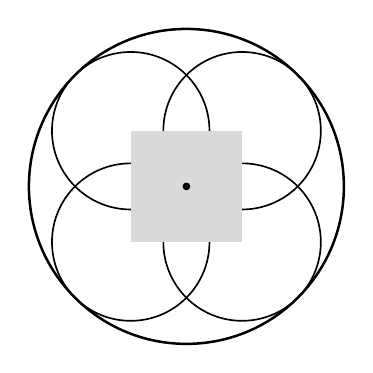
\begin{tikzpicture}[scale=2.0, semithick]
  \draw[line width=0.9pt] (0,0) circle[radius=1];
  \foreach \a in {45,135,225,315} {
    \draw (\a:0.5) circle[radius=0.5];
  }
  \fill[gray!30] (0.354,0.354) -- (0.354,-0.354) -- (-0.354,-0.354) -- (-0.354,0.354) -- cycle;
  \fill (0,0) circle (0.7pt);
\end{tikzpicture}
\end{center}
\nopagebreak[4]
\end{question}
\begin{question}
\gkti{10}函数 $f(x)=\dfrac{\sin x-1}{\sqrt{3-2\cos x-2\sin x}}$ 的值域是（　）

（A）$\left[-\dfrac{\sqrt2}2,0\right]$

（B）$[-1,0]$

（C）$[-\sqrt2,0]$

（D）$[-\sqrt3,0]$

\end{question}
\gkpart{二、填空题}

\begin{question}
\gkti{11}设集合 $U=\{1,2,3,4,5\}$，$A=\{2,4\}$，$B=\{3,4,5\}$，$C=\{3,4\}$，则 $(A\cup B)\cap(\complement_UC)=$\gkblank{}。

\end{question}
\begin{question}
\gkti{12}已知函数 $f(x)=\begin{cases}2x+3&(\text{\text{当} }x\neq0\text{ \text{时}})\\ a&(\text{\text{当} }x=0\text{ \text{时}})\end{cases}$ 在点 $x=0$ 处连续，则 $\lim\limits_{n\to\infty}\dfrac{an^2+1}{a^2n^2+n}=$\gkblank{}。

\end{question}
\begin{question}
\gkti{13}已知 $a^{\frac23}=\dfrac49$（$a>0$），则 $\log_{\frac23}a=$\gkblank{}。

\end{question}
\begin{question}
\gkti{14}设 $S_n$ 是等差数列 $\{a_n\}$ 的前 $n$ 项和，$a_{12}=-8$，$S_9=-9$，则 $S_{16}=$\gkblank{}。

\end{question}
\begin{question}
\gkti{15}直线 $l$ 与圆 $x^2+y^2+2x-4y+a=0$（$a<3$）相交于两点 $A$，$B$，弦 $AB$ 的中点为 $(0,1)$，则直线 $l$ 的方程为\gkblank{}。

\Needspace{0.4\textheight}
\end{question}
\begin{question}
\gkti{16}某人有 $4$ 种颜色的灯泡（每种颜色的灯泡足够多），要在如图所示的 $6$ 个点 $A$、$B$、$C$、$A_1$、$B_1$、$C_1$ 上各装一个灯泡，要求同一条线段两端的灯泡不同色，则每种颜色的灯泡都至少用一个的安装方法共有\gkblank{}种。（用数字作答）
\nopagebreak[4]
\begin{center}% 2008 年重庆卷理科第 16 题：三棱柱 ABC-A1B1C1 的 6 个顶点各装一个灯泡。
% 来源 PDF：gaokaomath-src/普通高考/2008/2008重庆理.pdf
% SHA-256：d3ca36cef73a00068b9c1a97ddb2f90bbc4f16b38459e380579090a02706d937
% 原页：2008重庆理.pdf 第 1 页（A3 三栏）第 2 栏，书页码 429。
% 绘制依据：按原页画出三棱柱的 9 条棱与 6 个顶点，A1B1C1 在下、ABC 在上。
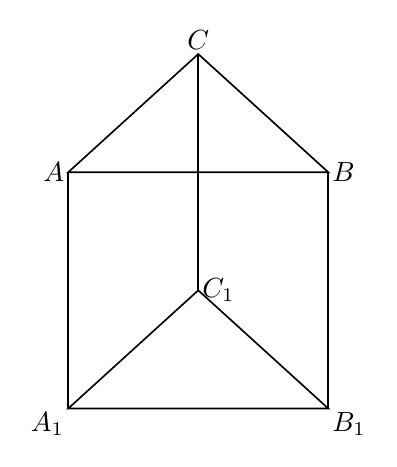
\begin{tikzpicture}[scale=1.5, semithick, every node/.style={inner sep=1.2pt}]
  \coordinate (A) at (0,2.0);
  \coordinate (B) at (2.2,2.0);
  \coordinate (C) at (1.1,3.0);
  \coordinate (A1) at (0,0);
  \coordinate (B1) at (2.2,0);
  \coordinate (C1) at (1.1,1.0);
  \draw (A) -- (B) -- (C) -- cycle;
  \draw (A1) -- (B1) -- (C1) -- cycle;
  \draw (A) -- (A1);
  \draw (B) -- (B1);
  \draw (C) -- (C1);
  \node[left] at (A) {$A$};
  \node[right] at (B) {$B$};
  \node[above] at (C) {$C$};
  \node[below left] at (A1) {$A_1$};
  \node[below right] at (B1) {$B_1$};
  \node[right] at (C1) {$C_1$};
\end{tikzpicture}
\end{center}
\nopagebreak[4]
\end{question}
\gkpart{三、解答题}

\begin{question}
\gkti{17}设 $\triangle ABC$ 的内角 $A$，$B$，$C$ 的对边分别为 $a$，$b$，$c$，且 $A=60^\circ$，$c=3b$。求：

（1）$\dfrac ac$ 的值；

（2）$\cot B+\cot C$ 的值。

\end{question}
\begin{question}
\gkti{18}甲、乙、丙三人按下面的规则进行乒乓球比赛：第一局由甲、乙参加而丙轮空，以后每一局由前一局的获胜者与轮空者进行比赛，而前一局的失败者轮空。比赛按这种规则一直进行到其中一人连胜两局或打满 $6$ 局时停止。设在每局中参赛者胜负的概率均为 $\dfrac12$，且各局胜负相互独立。求：

（1）打满 $3$ 局比赛还未停止的概率；

（2）比赛停止时已打局数 $\xi$ 的分布列与期望 $E\xi$。

\Needspace{0.4\textheight}
\end{question}
\begin{question}
\gkti{19}如图，在 $\triangle ABC$ 中，$B=90^\circ$，$AC=\dfrac{15}2$，$D$、$E$ 两点分别在 $AB$、$AC$ 上，使 $\dfrac{AD}{DB}=\dfrac{AE}{EC}=2$，$DE=3$。现将 $\triangle ABC$ 沿 $DE$ 折成直二角角，求：

（1）异面直线 $AD$ 与 $BC$ 的距离；

（2）二面角 $A-EC-B$ 的大小（用反三角函数表示）。
\nopagebreak[4]
\begin{center}% 2008 年重庆卷理科第 19 题：△ABC（B=90°）中 D∈AB、E∈AC，AD/DB=AE/EC=2，DE=3，
%   沿 DE 折成直二面角。
% 来源 PDF：gaokaomath-src/普通高考/2008/2008重庆理.pdf
% SHA-256：d3ca36cef73a00068b9c1a97ddb2f90bbc4f16b38459e380579090a02706d937
% 原页：2008重庆理.pdf 第 1 页（A3 三栏）第 3 栏，书页码 429。
% 绘制依据：左图为折叠前的直角三角形（DE ∥ BC），右图为折起后的立体图（虚线为折前的 DE 与 BC 位置）。
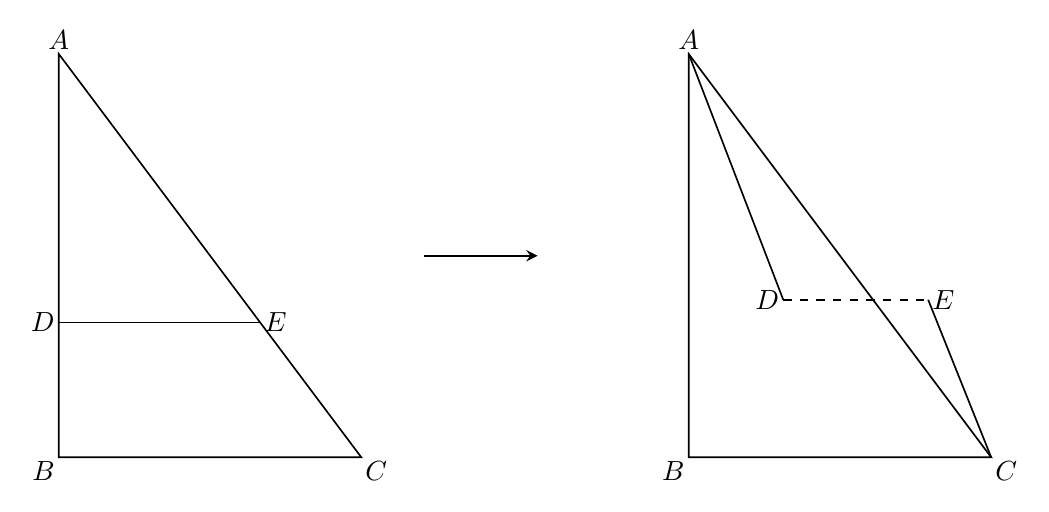
\begin{tikzpicture}[scale=1.6, semithick, every node/.style={inner sep=1.2pt}]
  % 左：折叠前
  \begin{scope}[shift={(0,0)}]
    \coordinate (B) at (0,0);
    \coordinate (C) at (2.4,0);
    \coordinate (A) at (0,3.2);
    \coordinate (D) at (0,1.07);
    \coordinate (E) at (1.6,1.07);
    \draw (A) -- (B) -- (C) -- cycle;
    \draw (D) -- (E);
    \node[below left] at (B) {$B$};
    \node[below right] at (C) {$C$};
    \node[above] at (A) {$A$};
    \node[left] at (D) {$D$};
    \node[right] at (E) {$E$};
  \end{scope}
  % 箭头
  \draw[->,>=stealth, line width=0.8pt] (2.9,1.6) -- (3.8,1.6);
  % 右：折起后
  \begin{scope}[shift={(5.0,0)}]
    \coordinate (B2) at (0,0);
    \coordinate (C2) at (2.4,0);
    \coordinate (A2) at (0,3.2);
    \coordinate (D2) at (0.75,1.25);
    \coordinate (E2) at (1.9,1.25);
    \draw (A2) -- (B2) -- (C2) -- cycle;
    \draw (A2) -- (D2);
    \draw[dashed] (D2) -- (E2);
    \draw (C2) -- (E2);
    \node[below left] at (B2) {$B$};
    \node[below right] at (C2) {$C$};
    \node[above] at (A2) {$A$};
    \node[left] at (D2) {$D$};
    \node[right] at (E2) {$E$};
  \end{scope}
\end{tikzpicture}
\end{center}
\nopagebreak[4]
\end{question}
\begin{question}
\gkti{20}设函数 $f(x)=ax^2+bx+c$（$a\neq0$），曲线 $y=f(x)$ 通过点 $(0,2a+3)$，且在点 $(-1,f(-1))$ 处的切线垂直于 $y$ 轴。

（1）用 $a$ 分别表示 $b$ 和 $c$；

（2）当 $bc$ 取得最小值时，求函数 $g(x)=-f(x)\mathrm e^{-x}$ 的单调区间。

\Needspace{0.4\textheight}
\end{question}
\begin{question}
\gkti{21}如图，$M(-2,0)$ 和 $N(2,0)$ 是平面上的两点，动点 $P$ 满足：$|PM|+|PN|=6$。

（1）求点 $P$ 的轨迹方程；

（2）若 $|PM|\cdot|PN|=\dfrac2{1-\cos\angle MPN}$，求点 $P$ 的坐标。
\nopagebreak[4]
\begin{center}% 2008 年重庆卷理科第 21 题：M(-2,0)、N(2,0)，动点 P 满足 |PM|+|PN|=6。
% 来源 PDF：gaokaomath-src/普通高考/2008/2008重庆理.pdf
% SHA-256：d3ca36cef73a00068b9c1a97ddb2f90bbc4f16b38459e380579090a02706d937
% 原页：2008重庆理.pdf 第 2 页（A3 三栏）第 2 栏，书页码 430。
% 绘制依据：按原页画坐标轴、M、N 与点 P，并连 PM、PN。
\begin{tikzpicture}[scale=0.95, semithick, every node/.style={inner sep=1.2pt}]
  \draw[->,>=stealth] (-3.4,0) -- (5.0,0) node[right] {$x$};
  \draw[->,>=stealth] (0,-2.6) -- (0,2.6) node[above] {$y$};
  \node[below left] at (0,0) {$O$};
  \coordinate (M) at (-2,0);
  \coordinate (N) at (2,0);
  \coordinate (P) at (3.4,1.6);
  \draw (M) -- (P) -- (N);
  \fill (M) circle (1.3pt); \node[below] at (M) {$M(-2,0)$};
  \fill (N) circle (1.3pt); \node[below] at (N) {$N(2,0)$};
  \fill (P) circle (1.3pt); \node[right] at (P) {$P$};
\end{tikzpicture}
\end{center}
\nopagebreak[4]
\end{question}
\begin{question}
\gkti{22}设各项均为正数的数列 $\{a_n\}$ 满足 $a_1=2$，$a_n=a_{n+1}^{\frac32}a_{n+2}$（$n\in\mathbf N^*$）。

（1）若 $a_2=\dfrac14$，求 $a_3$，$a_4$，并猜想 $a_{2008}$ 的值（不需证明）；

（2）记 $b_n=a_1a_2\cdots a_n$（$n\in\mathbf N^*$），若 $b_n\geqslant2\sqrt2$ 对 $n\geqslant2$ 恒成立，求 $a_2$ 的值及数列 $\{b_n\}$ 的通项公式。

\end{question}